% initial proposal of our wireless transfer system
%
%
Our major goal is to provide an efficient solution that best meets the challenges in battery charging systems using wireless power transfer.
Those challenges include:
\begin{enumerate}
\item \emph{Charging the battery as fast as possible}.
Batteries can store a large amount of charge, but the charging speed limit get smaller with smaller sized batteries. Exceeding the charging current limit will deteriorate the battery's life and is more likely to happen when using smaller batteries as they have a lower charging current limit. To overcome this difficulty we propose adding a supercapacitor parallelly with a battery. The supercapacitor will function as a small buffer for charging the battery as it can hold a smaller amount of charge compared to the same size battery. Using a powerfull combination of a battery in parallel with a supercapacitor will offer a much faster charging cycle as supercapacitors are know to charge fast and will provide a robuster system for they have a longer cycle life \cite{superbattery}, \cite{IAmp} as discussed in Section \ref{sec:prior}.

\item \emph{Ensuring a long battery life by creating a large charge to discharge ratio.}
In our scenario we don't want the user to be waiting for a longer time than 15 minutes for the wristband to charge. This introduces the need to store as much charging current in short intervals as possible. Batteries have a relatively low cycle life, making them unfit to be frequently charged and discharged. By positioning a supercapacitor in parallel with the battery, it acts as a buffer to store a large amount of charging current. Sequentially the same supercapacitor can use this current to charge the battery with a slow pace. This ensures a longer battery life in terms of a large charge to discharge ratio. 

\item \emph{Developing an efficient protocol for sharing the available charge.}
We don't want to develop a wastefull system in terms of energy. For this reason we want to propose an efficient protocol that enures the available energy is efficiently used. By using UML state and sequence diagram we will display the efficient flows of energy. Based on these diagram we will develop the protocols on an arduino to demonstrate our working fully functional system as will be discussed in Section \ref{sec:proto}.
\end{enumerate}

%----------- Schematics of the design of the system---------
\begin{figure}[h!]
\centering
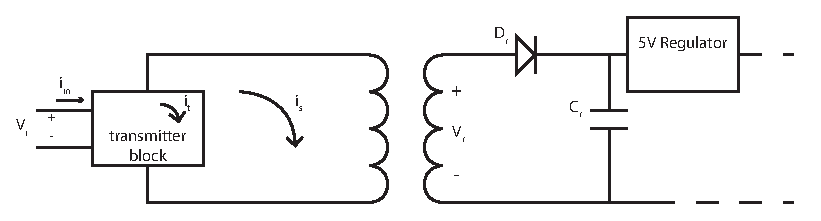
\includegraphics[width=0.8\textwidth]{design.pdf}
\caption{Design of the system}
\label{fig:design1}
\end{figure}

Figure \ref{fig:design1} represents the general framework of a wireless power transfer system as proposed in the assigned paper \cite{paper}. In order to propose a system design applicable to the subject of wireless power transfer we will use this framework and come up with our own parameters and design for the application. To charge the application with a wireless power transmitting system a regulated voltage of 5V with a maximum current of 300mA is required. Based on these specifications we found a wireless power transfer set online \cite{wireless} and purchased this set as seen in figure \ref{fig:set} to build our system with. The specifications of this set are mentioned on \cite{wireless}, but will be discussed more detailed in Section \ref{sec:results}. 

%-----------Our ordered set of wireless power transmitter-receiver-------------
\begin{figure}[h!]
\centering
\includegraphics[width=0.7\textwidth]{wirelessset.jpg}
\caption{Engineeringshock Electronics Wireless power transfer set}
\label{fig:set}
\end{figure}